\documentclass[11pt]{article}

\usepackage{enumerate}

\usepackage{fullpage}
\usepackage{framed}
\usepackage[numbers]{natbib}
\usepackage{dsfont}
\usepackage{latexsym}
\usepackage{amsmath}
\usepackage{amsthm}
\usepackage{amssymb}
\usepackage{amsfonts}
\usepackage{mathrsfs}
\usepackage{aliascnt}
\usepackage{siunitx}
% \usepackage{pstricks}
% \usepackage{pst-all}
% \usepackage{pstricks-add}
% \usepackage{pst-plot}
\usepackage{graphicx}
% \usepackage{subfig}
%\usepackage[margin=1in]{geometry}
% \usepackage{enumerate}
\usepackage[pdfpagelabels,pdfpagemode=None]{hyperref}
\usepackage{algorithmic}
\usepackage{algorithm}
\newcommand{\norm}[1]{\left\lVert #1 \right\rVert}
\usepackage{pdfpages}


\delimiterfactor=1100

\setlength{\delimitershortfall}{0pt}

\newcommand{\argmax}{\operatorname{arg\,max}}
\newcommand{\argmin}{\operatorname{arg\,min}}
\newcommand{\OPT}{\operatorname{OPT}}
\DeclareMathOperator{\MC}{MC}

\newtheorem{theorem}{Theorem}%

\newaliascnt{lemma}{theorem}
\newtheorem{lemma}[lemma]{Lemma}%
\aliascntresetthe{lemma}
\newtheorem*{rellemma}{Lemma}
\providecommand*{\lemmaautorefname}{Lemma}


\newtheorem{claim}{Claim}%
\newcommand{\claimautorefname}{Claim}

\newtheorem{corollary}{Corollary}%

\newtheorem{condition}{Condition}%
\newcommand{\conditionautorefname}{Cond.}

\newtheorem{proposition}{Proposition}%
\newcommand{\propositionautorefname}{Proposition}


\newtheorem{algo}{Algorithm}%
\def\algoautorefname{Algorithm}

\theoremstyle{definition}
\newtheorem{definition}{Definition}

\newtheorem{example}{Example}
\newcommand{\exampleautorefname}{Ex.}

\newtheorem{remark}{Remark}
\newcommand{\remarkautorefname}{Remark}

% \newenvironment{proofof}[1]{\vspace{0.1in} {\sc Proof of #1.}}{\hfill\qed}
% \newenvironment{proofsk}{\vspace{0.1in} {\sc Proof sketch.}}{\hfill\qed}


\def\algorithmautorefname{Algorithm}
\def\corollaryautorefname{Corollary}
\def\lemmaautorefname{Lemma}
\def\sectionautorefname{Section}
\def\subsectionautorefname{Section}
\def\defiautorefname{Definition}

\allowdisplaybreaks

% \input{notation}

\begin{document}
\begin{framed}
\begin{center}
\Large{\sc CPSC532W: Homework 1}
\end{center}
\hfill Name: Adam Jozefiak, Student No.: 27458158 

\end{framed}

\begin{enumerate}

% 1
\item We show that Gamma distribution is conjugate to the Poisson distribution. Let

$$\begin{array}{cc}
\lambda \sim \text{Gamma}(\alpha,\beta) \\ 
x_1,\ldots, x_N \sim \text{Poisson}(\lambda)
\end{array}$$

Then by Bayes rule, the posterior distribution $p(\lambda | \bf{x})$ can be written as 

$$p(\lambda | x_{1:N}) = \frac{p(x_{1:N}| \lambda)p(\lambda)}{p(x_{1:N})} \propto p(x_{1:N} | \lambda)p(\lambda)$$

where the last proportionallity follows by the fact that $p(x_{1:N}) = \int p(x_{1:N}|\lambda)p(\lambda)d\lambda$ is constant.

We note the probability density functions of  $\text{Gamma}(\alpha,\beta)$ and $\text{Poisson}(\lambda)$:

$$\begin{array}{c}
p(\gamma) = \frac{\beta^\alpha}{\Gamma(\alpha)}\lambda^{\alpha-1}e^{-\beta\lambda} \\ \\
p(x_{1:N}) = \prod_{i=1}^N\frac{\lambda^{x_i}e^{-\lambda}}{x_i!}
\end{array}$$

Then, 

$$\begin{array}{rcll}
p(\lambda | x_{1:N}) &  \propto & p(x_{1:N} | \lambda)p(\lambda) & \text{as argued earlier} \\ \\

& = & ( \prod_{i=1}^N\frac{\lambda^{x_i}e^{-\lambda}}{x_i!})( \frac{\beta^\alpha}{\Gamma(\alpha)}\lambda^{\alpha-1}e^{-\beta\lambda}) \\ \\

& = & \frac{\beta^\alpha}{\prod_{i=1}^Nx_i!}\lambda^{\sum_{i=1}^Nx_i + \alpha-1}e^{-(n+\beta)\lambda} \\ \\

&\propto & \lambda^{\sum_{i=1}^Nx_i + \alpha-1}e^{-(n+\beta)\lambda} &\text{ by $\lambda$ not appearing in $\frac{\beta^\alpha}{\prod_{i=1}^Nx_i!}$}\\ \\
\end{array}$$

Therefore, up to a normalizing constant, $p(\lambda | x_{i:N}) \propto \lambda^{\sum_{i=1}^Nx_i + \alpha-1}e^{-(n+\beta)\lambda} $ and hence $p(\lambda | x_{1:N}) \sim \text{ Gamma}(\sum_{i=1}^Nx_i + \alpha, n+\beta)$. Therefore, the a prior Gamma distribution is a conjugate prior for a likelihood Poisson distribution.

\item Let $x$ and $x'$ be vectors of random variables. Then the Gibbs transition operator, for the change in the $k^{\text{th}}$ variable or index of $x$, is defined as $T_k(x,x') = p(x_k' | x_{-k}) \prod_{i\neq k} \mathbb{I}(x_i = x_i')$. Then we can see that the Gibbs transition operator satisfies the detailed balance equattion by hte following argument

$$\begin{array}{rcll}
& & p(x)T(x,x') \\ \\

& = & p(x)p(x_k'|x_{-k})\prod_{i\neq k}\mathbb{I}(x_i = x_i') \\ \\

& = & p(x_k|x_{-k})p(x_{-k})p(x_k'|x_{-k})\prod_{i\neq k}\mathbb{I}(x_i = x_i') & \text{by the product rule}\\ \\ 

& = & p(x')p(x_k|x_{-k})\prod_{i\neq k}\mathbb{I}(x_i = x_i') & \text{by the product rule on $p(x') = p(x_k' |x_{-k})p(x_{-k})$}\\ \\ 

& = & p(x')p(x_k|x_{-k}')\prod_{i\neq k}\mathbb{I}(x_i = x_i') & \text{by $p(x_k|x_{-k})\prod_{i\neq k}\mathbb{I}(x_i = x_i') > 0 \Rightarrow x_{-k}'=x_{-k}$} \\ \\ 

& = & p(x')T(x',x)
\end{array}$$

This completes the proof of the Gibbs transition operator satisfying the detailed balance equation and therefore Gibbs transition operator can be interpreted as a Metropolis-Hastings transition operator that always accepts.

% 3
\item My solution to this problem is in Julia, based off the sample code. I found that the probability of it being cloudy given that the grass is wet is 57.58$\%$ by enumerating all possible world states and conditioning by counting which proportion are cloudy given the grass is wet. Using ancestral sampling and rejection, with 10000 successful samples, I found that the probability that it is cloudy given the grass is wet is 57.50$\%$ while 35.43$\%$ of samples were rejected. Using Gibbs sampling I found that the probability that it is cloudy given that the grass is wet is 58.66$\%$. In my implementation, an index of 2 indicates a ``true'' assignment and an index 1 indicates a ``false'' assignment to a random variable.

Below is my code for computing the probability by enumerating all possible world states and conditioning by counting which proportion are cloudy given the grass is wet:

\begin{center}
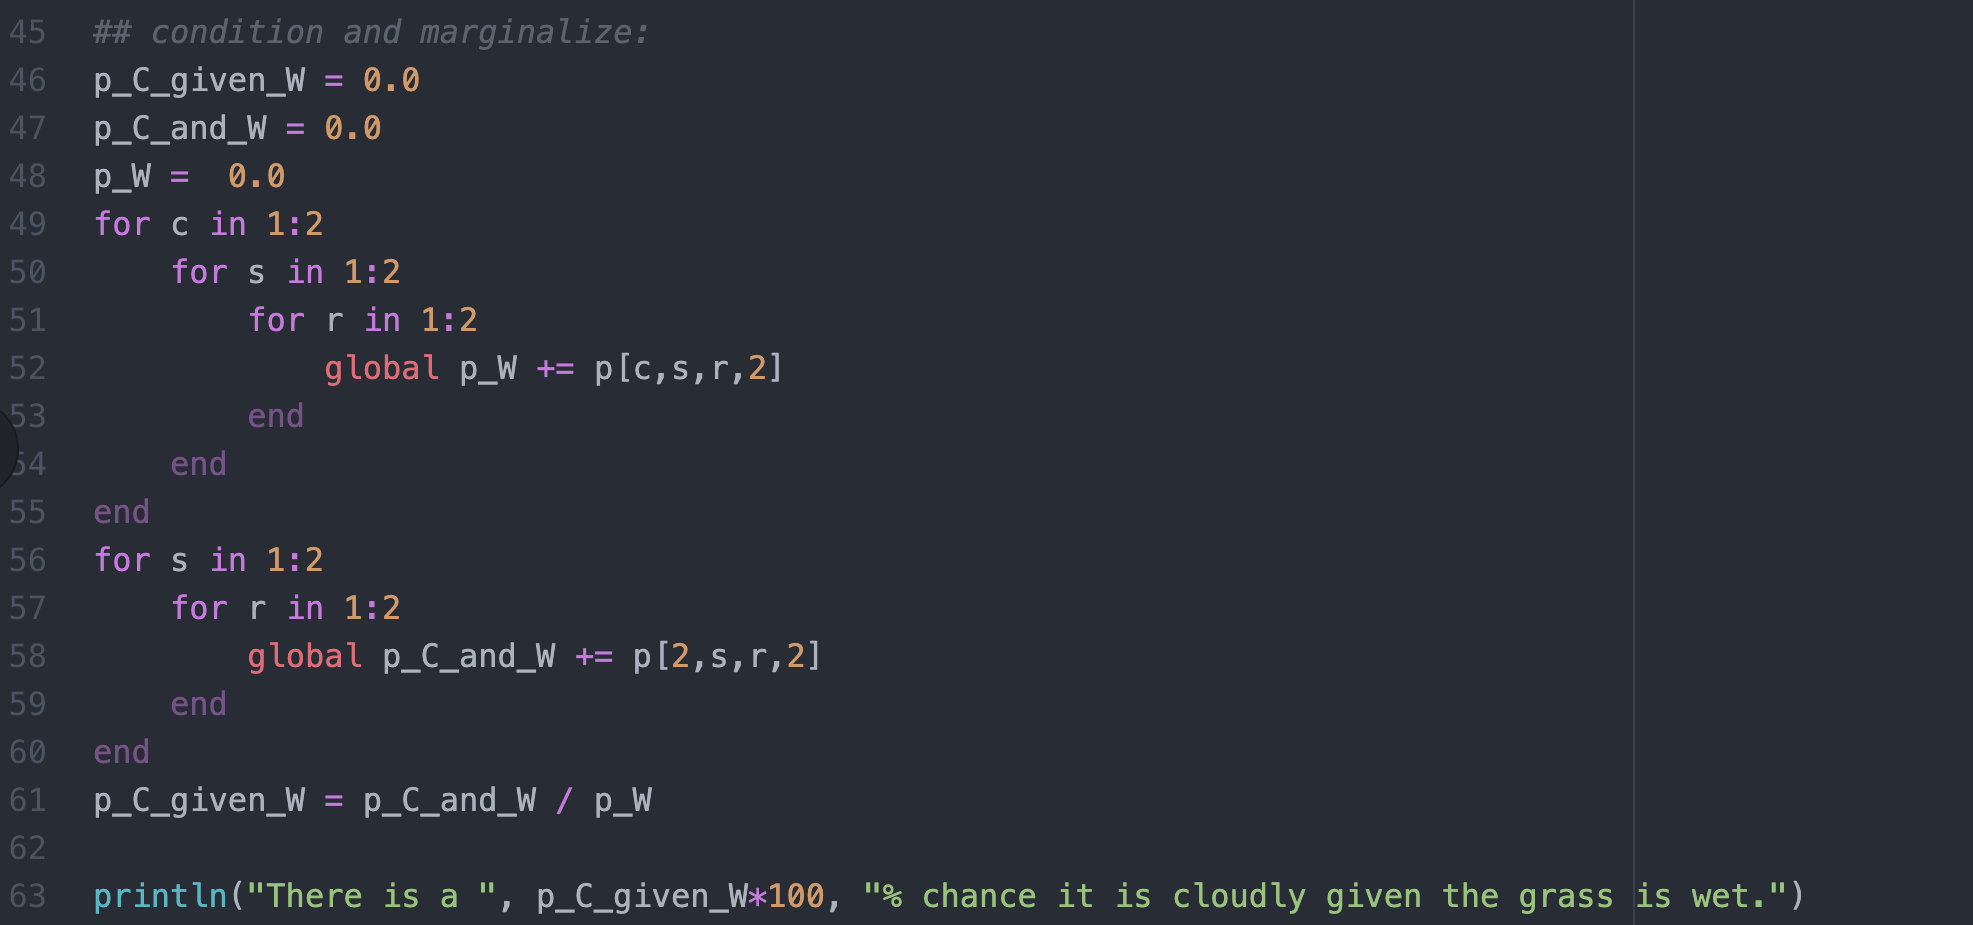
\includegraphics[scale=0.4]{figures/q3_1}
\end{center}

Below is my code for computing the probability by ancestral sampling and rejection:

\begin{center}
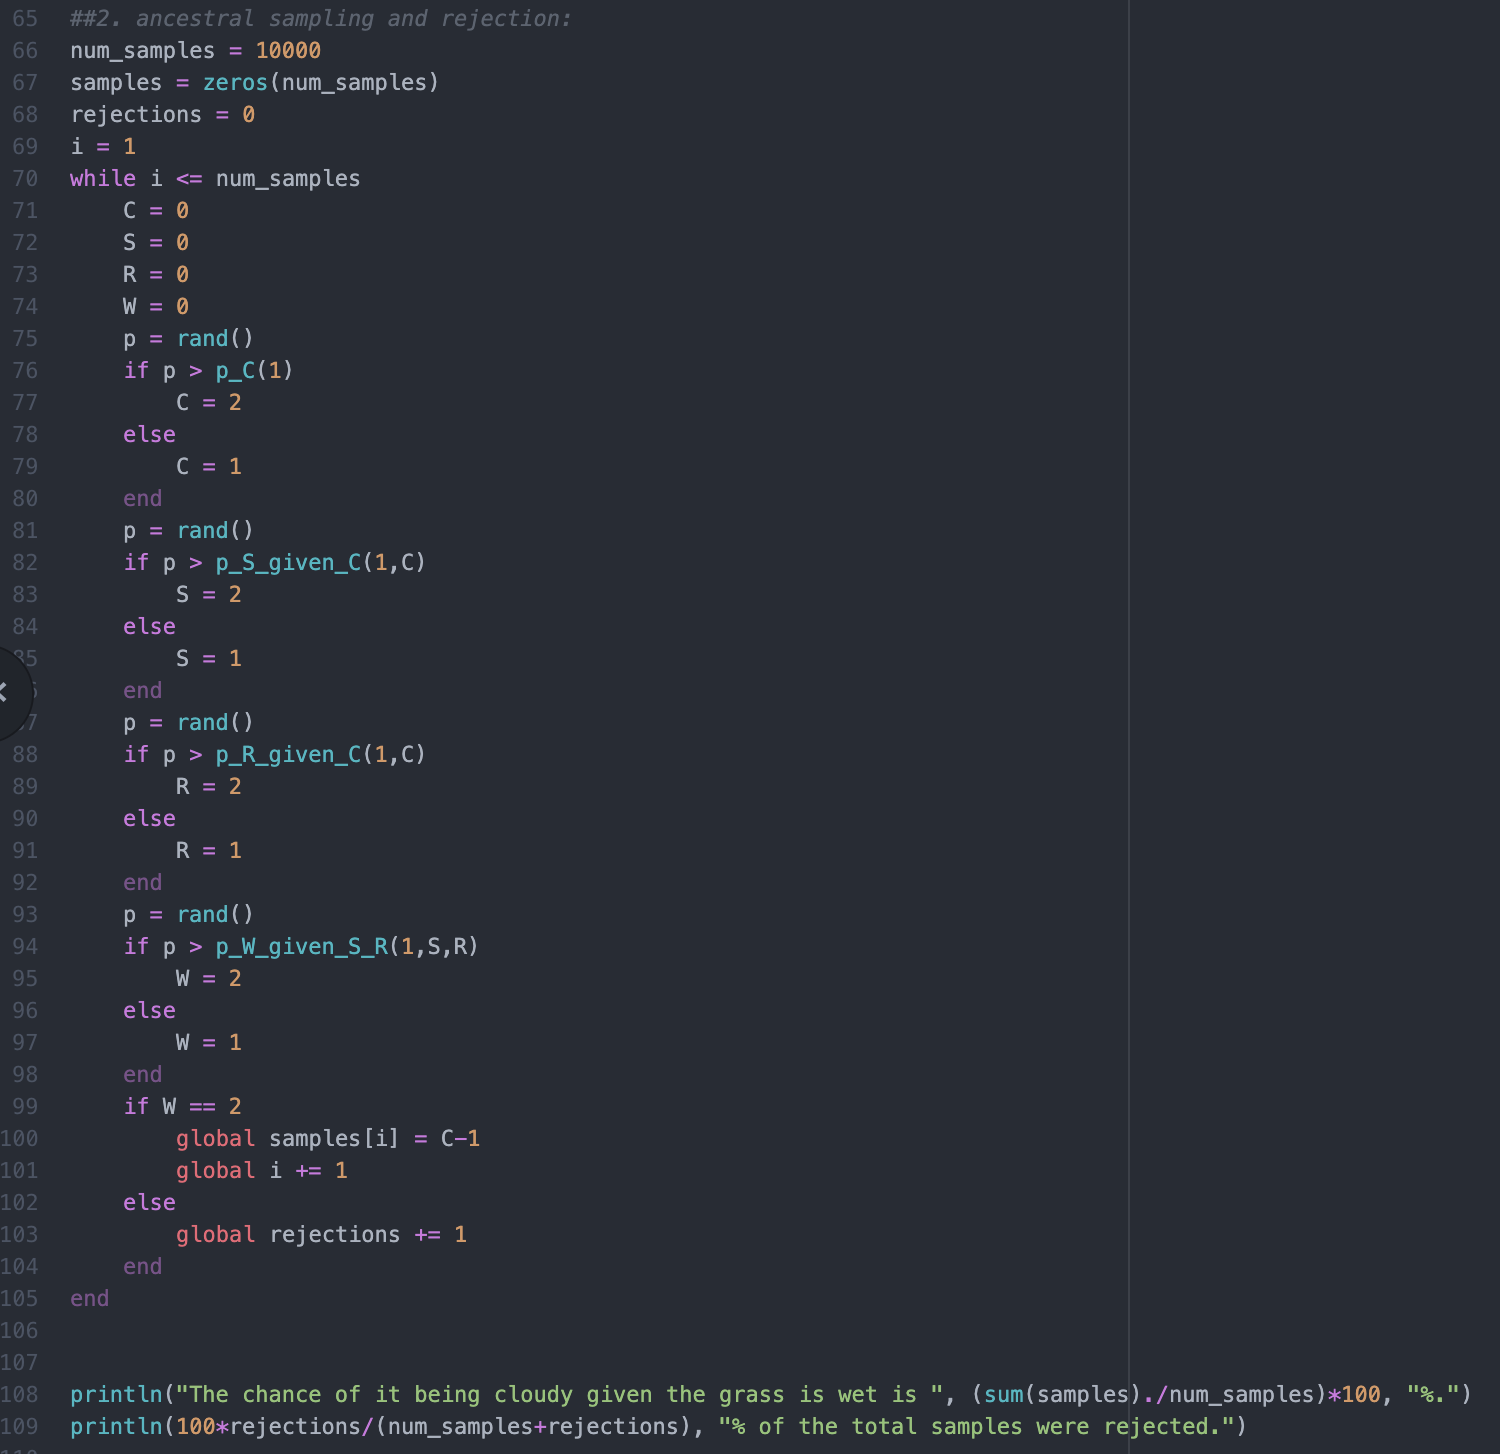
\includegraphics[scale=0.6]{figures/q3_2}
\end{center}

Below is my code for computing the probability by Gibbs sampling:

\begin{center}
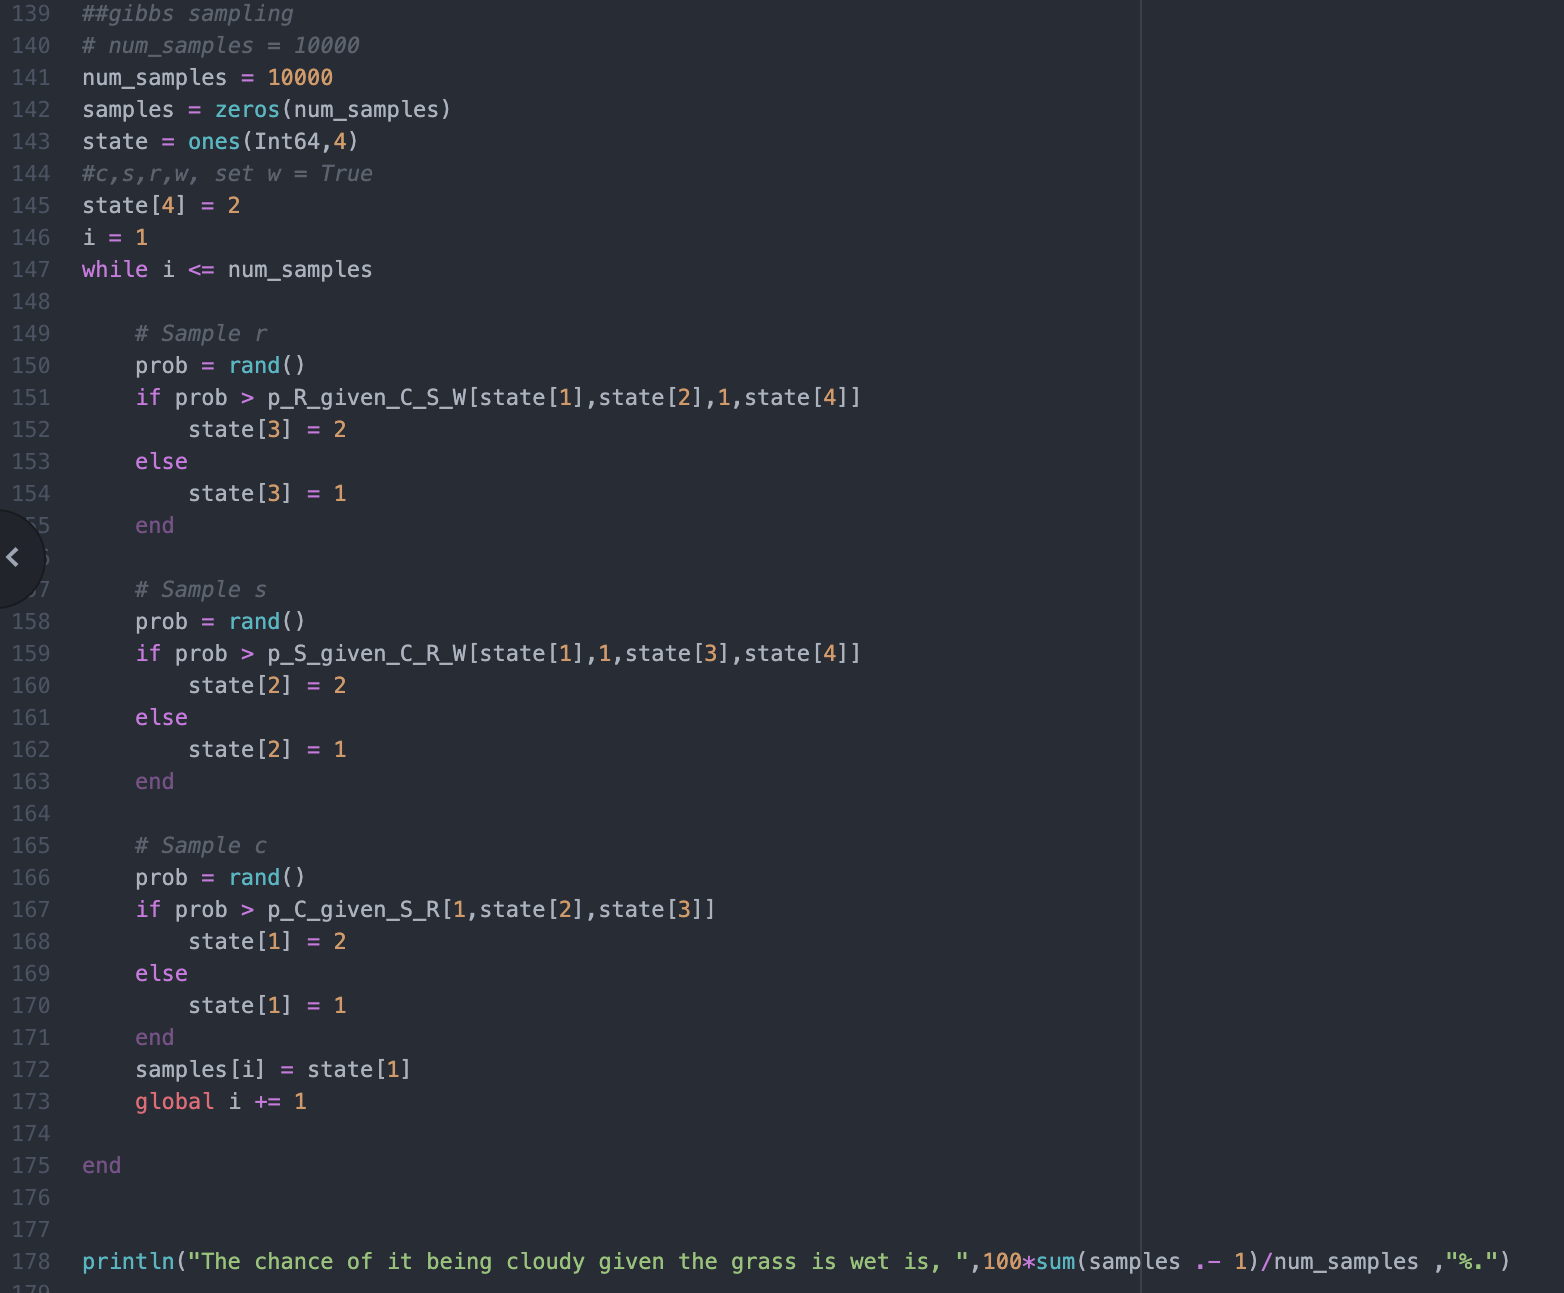
\includegraphics[scale=0.6]{figures/q3_3}
\end{center}


% 4
\item 

\begin{itemize}

\item We first derive the updates for Metropolis Hastings sampling of the $\hat{t}$ block, that is we want to sample from $p(\hat{t}|\hat{x},t,x,w,\sigma^2,\alpha)$. 

Let the proposal distribution be $\hat{t}'|\hat{t} \sim \text{ Normal}(\hat{t},\sigma^2)$. Then $\hat{t}'|\hat{t}$ and $\hat{t}|\hat{t}'$ are symmetric, i.e $q(\hat{t}'|\hat{t})=q(\hat{t}|\hat{t}')$, and so $\frac{q(\hat{t}|\hat{t}')}{q(\hat{t}'|\hat{t})} = 1$. Then after sampling $\hat{t}'$ from $q(\hat{t}'|\hat{t})$ the accepting probability is:

$$\begin{array}{rcll}

& & A(\hat{t}'|\hat{t}) \\ \\

& = & \min(1,\frac{p(\hat{t}'|\hat{x},t,x,w,\sigma^2,\alpha)q(\hat{t}|\hat{t}')}{p(\hat{t}|\hat{x},t,x,w,\sigma^2,\alpha)q(\hat{t}'|\hat{t})}) \\ \\

& = & \min(1,\frac{p(\hat{t}'|\hat{x},t,x,w,\sigma^2,\alpha)}{p(\hat{t}|\hat{x},t,x,w,\sigma^2,\alpha)}) & \text{by the symmetry of the proposal distribution} \\ \\

& = & \min(1, \frac{p(\hat{t}',\hat{x},t,x,w,\sigma^2,\alpha)p(\hat{x},t,x,w,\sigma^2,\alpha)}{p(\hat{t},\hat{x},t,x,w,\sigma^2,\alpha)p(\hat{x},t,x,w,\sigma^2,\alpha)}) & \text{by the product rule} \\ \\

& = & \min(1, \frac{p(\hat{t}',\hat{x},t,x,w,\sigma^2,\alpha)}{p(\hat{t},\hat{x},t,x,w,\sigma^2,\alpha)}) \\ \\

& = & \min(1, \frac{\prod_{i=1}^Np(t_i|x,w,\sigma^2)p(w|\alpha)p(\hat{t}'|\hat{x},w,\sigma^2)}{\prod_{i=1}^Np(t_i|x,w,\sigma^2)p(w|\alpha)p(\hat{t}|\hat{x},w,\sigma^2)}) \\ \\

& = & \min(1, \frac{p(\hat{t}'|\hat{x},w,\sigma^2)}{p(\hat{t}|\hat{x},w,\sigma^2)}) \\ \\

\end{array}$$

Therefore, in the Metropolis Hastings sampling block for $\hat{t}$, we sample $\hat{t}'$ from $\text{Normal}(\hat{t}, \sigma^2)$ and we accept $\hat{t}'$ with probability $\min(1, \frac{p(\hat{t}'|\hat{x},w,\sigma^2)}{p(\hat{t}|\hat{x},w,\sigma^2)})$.

Next, we derive the updates for Metropolis Hastings sampling of the $w$ block, that is we want to sample from $p(w|\hat{t}, \hat{x},t,x,\sigma^2,\alpha)$. We can treat the $\hat{t}$ and $\hat{x}$ as $t$ and $x$ and so we will derive the updates for Metropolis Hastings sampling of $p(w|t,x,\sigma^2,\alpha)$. 

Let the proposal distribution be $w'|w \sim \text{ Normal}(w,\alpha I)$. Then $w'|w$ and $w|w'$ are symmetric, i.e $q(w'|w)=q(w|w')$, and so $\frac{q(w|w')}{q(w'|w)} = 1$. Then after sampling $w'$ from $q(w'|w)$ the accepting probability is:

$$\begin{array}{rcll}

& & A(w'|w) \\ \\

& = & \min(1,\frac{p(w'|t,x,\sigma^2,\alpha)q(w|w')}{p(w|t,x,\sigma^2,\alpha)q(w'|w)}) \\ \\

& = & \min(1,\frac{p(w'|t,x,\sigma^2,\alpha)}{p(w|t,x,\sigma^2,\alpha)}) & \text{by the symmetry of the proposal distribution} \\ \\

& = & \min(1,\frac{p(w',t,x,\sigma^2,\alpha)p(t,x,\sigma^2,\alpha)}{p(w,t,x,\sigma^2,\alpha)p(t,x,\sigma^2,\alpha)})& \text{by the product rule} \\ \\

& = & \min(1,\frac{p(w',t,x,\sigma^2,\alpha)}{p(w,t,x,\sigma^2,\alpha)}) \\ \\

& = & \min(1, \frac{\prod_{i=1}^Np(t_i|x,w,\sigma^2)p(w|\alpha)}{\prod_{i=1}^Np(t_i|x,w',\sigma^2)p(w'|\alpha)}) \\ \\

\end{array}$$

Therefore, in the Metropolis Hastings sampling block for $w$, we sample $w'$ from $\text{Normal}(w, \alpha I)$ and we accept $w'$ with probability $\min(1, \frac{\prod_{i=1}^Np(t_i|x,w,\sigma^2)p(w|\alpha)}{\prod_{i=1}^Np(t_i|x,w',\sigma^2)p(w'|\alpha)})$.


\item To perform pure Gibbs sampling for $w$ and $\hat{t}$ we would like to first sample $w$ from $p(w|\hat{t},\hat{x},t,x,\sigma^2,\alpha)$. As argued earlier, we can treat $\hat{t}$ and $\hat{x}$ as being part of $t$ and $x$ and so we might as well sample $w$ from $p(w|t,x,\sigma^2,\alpha)$. Then we have that 

$$\begin{array}{rcll}
& & p(w |t,x,\sigma^2,\alpha) \\ \\

& = & \frac{p(w,t,x,\sigma^2,\alpha)}{p(t,x,\sigma^2,\alpha)} & \text{by the product rule} \\ \\

& \propto & p(w,t,x,\sigma^2,\alpha) \\ \\

& = & \prod_{i=1}^Np(t_i|x_i,w\sigma^2)p(w|\alpha)
\end{array}$$

Hence, in Gibbs sampling, we can sample $w$ proportionally to the joint distribution or specifically the distribution $\prod_{i=1}^Np(t_i|x_i,w\sigma^2)p(w|\alpha)$. As will be shown in the next bullet point, this distribution is the posterior of $w$ and it is 

$$w |t,x,\sigma^2,\alpha \sim \text{ Normal}([\frac{1}{\alpha}I+\frac{1}{\sigma^2}xx^T]^{-1}\frac{1}{\sigma^2}xt, [\frac{1}{\alpha}I+\frac{1}{\sigma^2}xx^T]^{-1})$$

Next, we need to sample $\hat{t}$ which requires sampling from $p(\hat{t}|\hat{x},t,x,w,\sigma^2,\alpha)$. We can see that

$$\begin{array}{rcll}
& & p(\hat{t}|\hat{x},t,x,w,\sigma^2,\alpha) \\ \\

& = & \frac{p(\hat{t},\hat{x},t,x,w,\sigma^2,\alpha)}{p(\hat{x},t,x,w,\sigma^2,\alpha)} & \text{by the product rule} \\ \\

& \propto & p(\hat{t},\hat{x},t,x,w,\sigma^2,\alpha) \\ \\

& = & \prod_{i=1}^Np(t_i|x_i,w,\sigma^2)p(w|\alpha)p(\hat{t}|\hat{x},w,\sigma^2) \\ \\

& \propto & p(\hat{t}|\hat{x},w,\sigma^2) 
\end{array}$$

Hence, Gibbs sampling, we can sample $\hat{t}$ proportionally to the distriubtion $p(\hat{t}|\hat{x},w,\sigma^2)$ which has distribution Normal$(w^T\hat{x},\sigma^2)$.

\item We compute the analytic form of the posterior predictive: $p(\hat{t} | \hat{x}, t,x,\sigma^2,\alpha)$. We begin by noting the following

$$\begin{array}{rcll}
& & p(\hat{t} | \hat{x}, t,x,\sigma^2,\alpha) \\ \\

& = & \int p(\hat{t} | \hat{x}, t,x,\sigma^2,w,\alpha)nt p(\hat{t},w | \hat{x}, t,x,\sigma^2,\alpha)dw & \text{by the sum rule} \\ \\

& = & \int p(\hat{t} | \hat{x}, t,x,\sigma^2,w,\alpha)p(w | \hat{x},t,x,\sigma^2,\alpha)dw & \text{by the product rule} \\ \\

& = & \int p(\hat{t} | \hat{x},\sigma^2,w)p(w | t,x,\sigma^2,\alpha)dw 

\end{array}$$

Where the last line above follows by the fact that $p(\hat{t} | \hat{x}, t,x,\sigma^2,w,\alpha) = p(\hat{t} | \hat{x},\sigma^2,w)$ and $p(w | \hat{x},t,x,\sigma^2,\alpha) = p(w | t,x,\sigma^2,\alpha)$, the latter following by the fact that $w$ can only have a dependency on $\hat{x}$ if $\hat{t}$ is known.

Next, we will argue that both $\hat{t} | \hat{x},\sigma^2,w$ and $w | t,x,\sigma^2,\alpha$ are Gaussian random variables. Firstly, $\hat{t} | \hat{x},\sigma^2,w \sim \text{ Normal}(w^T\hat{x}, \sigma^2)$ by the likelihood given in the question. 

As for $w | t,x,\sigma^2,\alpha$ we note that 

$$\begin{array}{c}
w | \alpha \sim \text{ Normal}(0,\alpha I) \\ \\

t| w,x,\sigma^2 \sim \text{ Normal}(w^Tx, \sigma^2) 
\end{array}$$

Then we note that

$$p(w | t,x,\sigma^2,\alpha) \propto p(t | w, x,\sigma^2,\alpha)p(w,x|\sigma^2,\alpha) \propto p(t | w, x,\sigma^2)p(w|\alpha)$$

Then by 2.116, page 93,  in Pattern Recognition and MAchine Learning by Bishop it follows that

$$w |t,x,\sigma^2,\alpha \sim \text{ Normal}([\frac{1}{\alpha}I+\frac{1}{\sigma^2}xx^T]^{-1}\frac{1}{\sigma^2}xt, [\frac{1}{\alpha}I+\frac{1}{\sigma^2}xx^T]^{-1})$$

Then by the earlier observations that 

$$\begin{array}{rcl}

p(\hat{t} | \hat{x}, t,x,\sigma^2,\alpha) & = & \int p(\hat{t} | \hat{x},\sigma^2,w)p(w | t,x,\sigma^2,\alpha)dw \\ \\

& \text{and} & \\ \\

\hat{t} | \hat{x},\sigma^2,w & \sim & \text{ Normal}(w^T\hat{x}, \sigma^2)

\end{array}$$

and by linear combination rules of Gaussian random variables we have that

$$\hat{t} | \hat{x}, t,x,\sigma^2,\alpha \sim \text{ Normal}([(\frac{1}{\alpha}I+\frac{1}{\sigma^2}xx^T)^{-1}\frac{1}{\sigma^2}xt]^T\hat{x}, \hat{x}^T(\frac{1}{\alpha}I+\frac{1}{\sigma^2}xx^T)^{-1}\hat{x}+\sigma^2)$$

This completes the derivation of the analytic for mof hte posterior predictive.

\end{itemize}

% 5
\item

\end{enumerate}

\end{document}
